\lecture{5}

In case of set theory, we had a notion of `cardinality' of a set. With the help of this notion, we can say that if two sets are isomorphic (set theoretically) then they have the same cardinality. But in case of topological spaces, we don't have any such quantity \ie\ we don't have any property which can tell us that two topological spaces are `homeomorphic' or not.

Building on this idea, we had classified sets into different types based on their cardinality like finite, countable, uncountable, etc. But in case of topology, classification of topological spaces is an open problem.

\section{Topological Properties I: Separation Axioms}

\begin{definition}[T1 Space]\label{def:t1_space}
	A topological space \((M, \O)\) is called \emph{T1} if for any two distinct points \(p, q \in M\) (\ie\ \(p \neq q\)), then
	\begin{equation}
		\exists U_p \in \O: q \notin U_p \label{eq:separation_axiom_t1}
	\end{equation}
	here \(U_p\) is an open neighbourhood of \(p\).
\end{definition}

\begin{definition}[T2 Space]\label{def:t2_space}
	A topological space \((M, \O)\) is called \emph{T2} or \emph{Hausdorff} if for any two distinct points \(p, q \in M\) (\ie\ \(p \neq q\)), then
	\begin{equation}
		\exists U_p, V_q \in \O: U_p \cap V_q = \0 \label{eq:separation_axiom_t2}
	\end{equation}
	here \(U_p\) and \(V_q\) are open neighbourhoods of \(p\) and \(q\) respectively.
\end{definition}
Intuitively, we can see why \cref{def:t1_space} and \cref{def:t2_space} are called `separation axioms'. Consider standard topology on \(\R^2\), see \cref{fig:separation_axioms}.
\begin{figure}[H]
	\centering
	\begin{subfigure}{0.45\textwidth}
		\centering
		\includegraphics[width=0.5\linewidth]{lec05-t1_intuition.png}
		\caption{T1 Space}
		\label{fig:t1_space}
	\end{subfigure}
	\begin{subfigure}{0.45\textwidth}
		\centering
		\includegraphics[width=0.6\linewidth]{lec05-t2_intuition.png}
		\caption{T2 Space}
		\label{fig:t2_space}
	\end{subfigure}
	\caption{Separation Axioms}
	\label{fig:separation_axioms}
\end{figure}

\begin{remark}[T1 vs T2]
	Every T2 space is a T1 space, but the converse is not true.
\end{remark}

\begin{example}
	Some examples of topological spaces based on separation axioms are:
	\begin{enumerate}[(a)]
		\item \(\R^d\) with standard topology is a T2 space.
		\item Zariski topology (algebraic geometry) is T1 but not T2.
		\item Chaotic topology is neither T1 nor T2.
		\item Discrete topology is always T1 and T2.
	\end{enumerate}
\end{example}


There are many other ``T'' properties, like T3, T4, etc. All of them have use cases in some area of mathematics or physics.
\begin{remark}[T$2\frac{1}{2}$ Space]
	A topological space \((M, \O)\) is called \emph{T$2\frac{1}{2}$} if for any two distinct points \(p, q \in M\) (\ie\ \(p \neq q\)), then there exists a closed neighbourhood \(U_p\) of \(p\) such that \(q \notin U_p\).
\end{remark}

\begin{theorem}[Uniqueness of Limit Point]\label{thm:uniqueness_limit_point}
	Let \((M, \O)\) be a Hausdorff space. Then every convergent sequence in \(M\) has a unique limit point.
\end{theorem}

\section{Compactness and Paracompactness}

Before we define compactness, we need to understand the concept of `open cover'.

\begin{definition}[Cover and Open Cover]\label{def:cover}
	Let \((M, \O)\) be a topological space. A set \(C \subseteq \powerset(M)\) is called a \emph{cover} of \(M\) if
	\begin{equation}
		\bigcup C = M. \label{eq:cover}
	\end{equation}
	If \(C \subseteq \O\) then it is called an \emph{open cover}.
\end{definition}

\begin{definition}[Subcover and Finite Subcover]\label{def:subcover}
	Let \(C\) be a cover of \(M\). A subset \(\tilde{C} \subseteq C\) is called a \emph{subcover} of \(C\) if
	\begin{equation}
		\bigcup \tilde{C} = M. \label{eq:subcover}
	\end{equation}
	If \(\tilde{C}\) is finite then it is called a \emph{finite subcover}.
\end{definition}

\subsection{Compactness}
\begin{definition}[Compact Space]\label{def:compact_space}
	A topological space \((M, \O)\) is called \emph{compact} if every open cover of \(M\) has a finite subcover.
\end{definition}

It is clear from the definition that compactness is a topological property. So we have,
\begin{remark}
	Let \((M, \O_M)\) and \((N, \O_N)\) be two homeomorphic topological spaces. Then \(M\) is compact if and only if \(N\) is compact.
\end{remark}

\begin{definition}[Compact Subset]\label{def:compact_subset}
	Let \((M, \O)\) be a topological space. A subset \(N \subseteq M\) is called \emph{compact} if the induced topology \((N, \eval{\O}_N)\) is compact.
\end{definition}

Determining whether a topological space is compact or not, is not an easy task. With the help of a suitable homeomorphism we can simplify this task.

\begin{theorem}[Heine-Borel Theorem]\label{thm:heine_borel}
	Let \((\R^d, \Ostd)\) be a topological space. Then a subset \(K \subseteq \R^d\) is compact if and only if it is closed and bounded.
\end{theorem}

\begin{remark}[Bounded Set in \(\R^d\)]
	A set \(K \subseteq \R^d\) is called \emph{bounded} if
	\begin{equation}
		\exists r > 0: K \subseteq B_r(0) \label{eq:bounded_set}
	\end{equation}
\end{remark}

We can extend \nameref{thm:heine_borel} to any metric space. But first we need to define the concept of `metric space'.

\begin{definition}[Metric Space]
	Let \(M\) be a set. A function \(d: M \times M \to \R\) is called a \emph{metric} on \(M\) if it satisfies the following properties for all \(p, q, r \in M\):
	\begin{itemize}
		\item \uline{\emph{Symmetry}:} \(d(p, q) = d(q, p)\).
		\item \uline{\emph{Positivity}:} \(d(p, q) \geq 0\) and \(d(p, q) = 0 \iff p = q\).
		\item \uline{\emph{Triangle Inequality}:} \(d(p, q) + d(q, r) \geq d(p, r)\).
	\end{itemize}
	A set \(M\) equipped with a metric \(d\) is called a \emph{metric space}.
\end{definition}

We can define `metric-induced topology' on a metric space as we did for \(\R^d\).

\begin{remark}[Metric-Induced Topology]
	Let \((M, d)\) be a metric space. Then the set \(B_r(p)\) is an open ball of radius \(r \in \R^+\) centered at \(p \in M\) defined as
	\begin{equation}
		B_r(p) = \{q \in M: d(p, q) < r\}. \label{eq:open_ball}
	\end{equation}
	With this, we can define the metric-induced topology \(\O_d\) on \(M\) as
	\begin{equation}
		U \in \O_d :\iff \forall p \in U, \exists r \in \R^+: B_r(p) \subseteq U. \label{eq:metric_induced_topology}
	\end{equation}
\end{remark}

\begin{theorem}[Generalized Heine-Borel Theorem]\label{thm:generalized_heine_borel}
	Let \((M, d)\) be a metric space with metric-induced topology \(\O_d\). Then a subset \(K \subseteq M\) is compact if and only if it is \emph{complete} and \emph{totally bounded}.
\end{theorem}

\begin{example}
	Example of compact subsets in \(\R\) are:
	\begin{enumerate}[(a)]
		\item \([0, 1]\) is compact in \((\R, \Ostd)\).

		\item \(\R\) is not compact in \((\R, \Ostd)\). It suffices to show that there exists an open cover of \(\R\) which does not have a finite subcover. Consider the open cover
		      \begin{equation}
			      C := \qty{(n, n + 1) \mid n \in \Z} \cup \qty{(n + \fhalf, n + \flatfrac{3}{2}) \mid n \in \Z}.
		      \end{equation}
	\end{enumerate}
\end{example}

\noindent We can prove that the product of two compact spaces is compact for product topology.
\begin{theorem}
	Let \((M, \O_M)\) and \((N, \O_N)\) be two compact topological spaces. Then the product space \((M \times N, \O_{M \times N})\) is compact.
\end{theorem}
Now extending this to finite product spaces is easy.

Compactness is a very strong property, and sometimes it doesn't hold. So we need a weaker property which can be used in such cases. This is where the concept of `paracompactness' comes in.

\subsection{Paracompactness}

\begin{definition}[Refinement of a Cover]\label{def:refinement_cover}
	Let \(C\) be a cover of \(M\). A cover \(R\) of \(M\) is called a \emph{refinement} of \(C\) if
	\begin{equation}
		\forall \tilde{U} \in R: \exists U \in C: \tilde{U} \subseteq U. \label{eq:refinement_cover}
	\end{equation}
	A refinement \(R\) is said to be:
	\begin{itemize}
		\item \emph{open} if \(R \subseteq \O\).
		\item \emph{Locally finite} if for every \(p \in M\), there exists an open neighbourhood \(U_p\) of \(p\) such that
		      \begin{equation}
			      \abs{\qty{\tilde{U} \in R \mid \tilde{U} \cap U_p \neq \0}} < \infty. \label{eq:locally_finite_cover}
		      \end{equation}
	\end{itemize}
\end{definition}

\begin{remark}
	Let \(C\) be a cover of \(M\) and let \(\tilde{C}\) be a subcover of \(C\). Then \(\tilde{C}\) is a refinement of \(C\). But the converse is not true.
\end{remark}

\begin{definition}[Paracompact Space]\label{def:paracompact_space}
	A topological space \((M, \O)\) is called \emph{paracompact} if every open cover of \(M\) has a locally finite open refinement.
\end{definition}

\begin{corollary}
	Every compact space is paracompact.
\end{corollary}

\begin{definition}[Metrisable Space]
	A topological space \((M, \O)\) is called \emph{metrizable} if there exists a metric \(d\) on \(M\) such that the metric-induced topology \(\O_d\) is same as \(\O\).
\end{definition}

\begin{theorem}[Stone's Theorem]\label{thm:stone}
	Every metrizable space is paracompact.
\end{theorem}

\begin{example}
	Let's see some topological spaces which are paracompact or not:
	\begin{enumerate}[(a)]
		\item The topological space \((\R^d, \Ostd)\) is metrizable since \(\Ostd = \O_d\) where \(d = \norm{\cdot}_2\). Hence, \((\R^d, \Ostd)\) is paracompact.
		\item Alexandroff Long Line is not paracompact. To construct it, we first observe that we could ``build'' \(\R\) by taking the interval \([0,1)\) and stacking countably many copies of it one after the other. Hence, in a sense, \(\R\) is equivalent to \(\Z \times [0,1)\). The long line \(L\) is defined analogously as \(L: \omega_1 \times [0,1)\), where \(\omega_1\) is an uncountable infinite set. The resulting space \(L\) is not paracompact.
	\end{enumerate}
\end{example}

\begin{theorem}
	Let \((M, \O)\) be a paracompact space and \((N, \O_N)\) be a compact space. Then the product space \((M \times N, \O_{M \times N})\) is paracompact.
\end{theorem}

\begin{corollary}
	Let \((M, \O)\) be a paracompact space and \((N_i, \O_{N_i})\) be compact spaces for all \(i \in \qty{1, 2, \ldots, n}\). Then the product space \(M \times N_1 \times N_2 \times \ldots \times N_n\) is paracompact.
\end{corollary}

At this point, we can discuss the sufficient and necessary criteria for paracompactness which are used as definitions in some books. For that we need to define the concept of `\emph{partition of unity}.'

\begin{definition}[Partition of Unity]\label{def:partition_of_unity}
	Let \((M, \O)\) be a topological space. A set \(\mathcal{F}\) of continuous functions \(\phi: M \to [0, 1]\) is called a \emph{partition of unity} if for each \(p \in M\),
	\begin{enumerate}[(a)]
		\item There exists an open neighbourhood \(U_p\) such that \(\phi(p) \ne 0\) for finitely many \(\phi \in \mathcal{F}\).
		\item \(\sum\limits_{\phi \in \mathcal{F}} \phi(p) = 1\).
	\end{enumerate}
\end{definition}

\begin{definition}[Partition of Unity Subordinate to a Cover]\label{def:partition_of_unity_subordinate}
	Let \((M, \O)\) be a topological space and let \(C\) be a cover of \(M\). A partition of unity \(\mathcal{F}\) is said to be \emph{subordinate} to \(C\) if:
	\begin{equation}
		\forall \phi \in \mathcal{F}: \exists U \in C: f(p) \ne 0 \implies p \in U. \label{eq:partition_of_unity_subordinate}
	\end{equation}
\end{definition}

\begin{theorem}
	Let \((M, \O)\) be a Hausdorff space. Then \(M\) is paracompact if and only if every open cover \(C\) admits a partition of unity subordinate to \(C\).
\end{theorem}

\begin{example}
	Let \((\R, \Ostd)\) be a topological space. By \cref{thm:stone}, \((\R, \Ostd)\) is paracompact. Consider the open cover \(C := \qty{U_1 = (-\infty, 1), U_2 = (0, \infty)}\). We can construct a partition of unity \(\mathcal{F} = \qty{\phi_1, \phi_2}\) subordinate to \(C\) as follows:
	\begin{align*}
		\phi_1(x) = \begin{cases}
			            1       & \text{if}\ x \le 0       \\
			            1 - x^2 & \text{if}\ 0 \le x \le 1 \\
			            0       & \text{if}\ x \ge 1
		            \end{cases} \qquad \text{and} \qquad
		\phi_2(x) = \begin{cases}
			            0   & \text{if}\ x \le 0       \\
			            x^2 & \text{if}\ 0 \le x \le 1 \\
			            1   & \text{if}\ x \ge 1
		            \end{cases}
	\end{align*}
	For \(\phi_1\), we have \(U_1 = (-\infty, 1)\) for which \(\phi_1(x) \ne 0\) and for \(\phi_2\), we have \(U_2 = (0, \infty)\) for which \(\phi_2(x) \ne 0\). Also, \(\phi_1(x) + \phi_2(x) = 1\) for all \(x \in \R\).
\end{example}

\section{Connectedness and Path-Connectedness}

\subsection{Connectedness}
\begin{definition}[Connected Space]\label{def:connected_space}
	A topological space \((M, \O)\) is called \emph{connected} unless there exists two non-empty open sets \(A, B\) such that
	\begin{equation}
		A \cup B = M \quad \text{and} \quad A \cap B = \0. \label{eq:connected_space}
	\end{equation}
\end{definition}

\begin{example}
	Let \(\qty(M := \R \setminus \qty{0}, \O := \eval{\Ostd}_{\R \setminus \qty{0}})\) be a topological space. Then \(M\) is not connected since we can write \(M = A \cup B\) where \(A = (-\infty, 0)\) and \(B = (0, \infty)\) with \(A \cap B = \0\).
\end{example}

\begin{theorem}
	The closed interval \([0, 1]\) with induced topology from \((\R, \Ostd)\) is connected.
\end{theorem}

\begin{theorem}
	Let \((M, \O)\) be a topological space. Then \(M\) is connected if and only if \(\0\) and \(M\) are the only subsets of \(M\) that are both open and closed.
\end{theorem}

\begin{proof}

	[\(\implies\)]:\\
	Suppose not there exists a set \(U \subseteq M\) that is both open and closed and \(U \neq \0, M\). Then \(M = U \dcup (M \setminus U)\). Since \(U\) is open and \(M \setminus U\) is open (as \(U\) is closed). Hence, \(M\) is not connected. \(\contra\)

	\noindent [\(\impliedby\)]:\\
	Suppose not \(M\) is not connected. Then there exists two non-empty open sets \(A, B\) such that \(A \cup B = M\) and \(A \cap B = \0\). Clearly, \(A \ne M\), if not then \(B = \0\). Since \(A\) is open, \(M \setminus A\) is closed. But \(M \setminus A = B\) is also open. Hence, \(B \ne \0, M\) is open and closed. \(\contra\)
\end{proof}

\subsection{Path-Connectedness}
\begin{definition}[Path-Connected Space]\label{def:path_connected_space}
	A topological space \((M, \O)\) is called \emph{path-connected} if for every pair of points \(p, q \in M\), there exists a continuous curve \(\gamma: [0, 1] \to M\) such that \(\gamma(0) = p\) and \(\gamma(1) = q\).
\end{definition}

\begin{example}
	Let \((\R^d, \Ostd)\) be a topological space. Then \((\R^d, \Ostd)\) is path-connected.
\end{example}
\begin{proof}
	Let \(p, q \in \R^d\). Then the curve \(\gamma(\lambda) := (1 - \lambda)p + \lambda q\) is continuous and \(\gamma(0) = p\) and \(\gamma(1) = q\).
\end{proof}

\begin{example}
	Let \(S := \qty{\qty(x, \sin(\frac{1}{x})) \mid x \in (0, 1]} \cup \qty{(0, 0)} \subseteq \R^2\). Then \((S, \eval{\Ostd}_{S})\) is not path-connected but connected.
	\begin{figure}[H]
		\centering
		\includegraphics[width = 0.7\textwidth]{lec05-eg_path_connected.png}
		% \caption{}
		% \label{fig:}
	\end{figure}
\end{example}

\begin{theorem}
	Every path-connected space is connected.
\end{theorem}
\begin{proof}
	Let \((M, \O)\) be a path-connected space. Suppose not \(M\) is not connected. Then there exists two non-empty open sets \(A, B\) such that \(A \dcup B = M\). Since, \(A\) and \(B\) are non-empty, we can choose \(a \in A\) and \(b \in B\). Since \(M\) is path-connected, there exists a continuous curve \(\gamma: [0, 1] \to M\) such that \(\gamma(0) = a\) and \(\gamma(1) = b\). Moreover, \(\gamma\) is continuous and \(A, B\) are open, disjoint sets, \(\preimg_{\gamma}(A)\) and \(\preimg_{\gamma}(B)\) are open, disjoint sets. We know
	\begin{equation*}
		\qty[0, 1] = \preimg_{\gamma}(M) = \preimg_{\gamma}(A \dcup B) = \preimg_{\gamma}(A) \dcup \preimg_{\gamma}(B).
	\end{equation*}
	Thus, existence of \(\preimg_{\gamma}(A)\) and \(\preimg_{\gamma}(B)\) implies that \([0, 1]\) is not connected. \(\contra\)
\end{proof}

\section{Homotopic Curves and Fundamental Group}

\begin{definition}[Homotopic Curves]\label{def:homotopic_curves}
	Let \((M, \O)\) be a topological space. Two continuous curves \(\gamma_1, \gamma_2: [0, 1] \to M\) such that
	\begin{equation*}
		\gamma_1(0) = \gamma_2(0) \quad \text{and} \quad \gamma_1(1) = \gamma_2(1)
	\end{equation*}
	are called \emph{homotopic} if there exists a continuous function \(h: [0, 1] \times [0, 1] \to M\) such that for all \(\lambda \in [0, 1]\),
	\begin{equation}
		h(0, \lambda) = \gamma_1(\lambda) \quad \text{and} \quad h(1, \lambda) = \gamma_2(\lambda). \label{eq:homotopic_curves}
	\end{equation}
\end{definition}
\uline{Intuitively}, two curves are homotopic if one can be continuously deformed into the other.\\
Pictorially, see \cref{fig:homotopic_curves}.
\begin{figure}[H]
	\centering
	\includegraphics[width=0.4\textwidth]{lec05-homotopic_curves.png}
	\caption{Homotopic Curves}
	\label{fig:homotopic_curves}
\end{figure}

\begin{proposition}[Homotopy is an Equivalence Relation]\label{prop:homotopy_equivalence_relation}
	Let \((M, \O)\) be a topological space. Define a relation \(\sim\) on the set of continuous curves \(\qty{\gamma: [0, 1] \to M}\) by
	\begin{equation}
		\gamma_1 \sim \gamma_2 :\iff \gamma_1 \text{ and } \gamma_2 \text{ are homotopic}. \label{eq:homotopy_equivalence_relation}
	\end{equation}
	Then \(\sim\) is an equivalence relation.
\end{proposition}
\begin{proof}
	Let \(\gamma_1, \gamma_2, \gamma_3: [0, 1] \to M\) be continuous curves.
	\begin{enumerate}[(a)]
		\item \uline{Reflexivity:} Define a continuous function \(h: [0, 1] \times [0, 1] \to M\) as \(h(t, \lambda) := \gamma_1(\lambda)\). Then \(h(0, \lambda) = \gamma_1(\lambda)\) and \(h(1, \lambda) = \gamma_1(\lambda)\) for all \(\lambda \in [0, 1]\). Hence, \(\gamma_1 \sim \gamma_1\).
		\item \uline{Symmetry:} Let \(\gamma_1 \sim \gamma_2\). Then there exists a continuous function \(h: [0, 1] \times [0, 1] \to M\) such that \(h(0, \lambda) = \gamma_1(\lambda)\) and \(h(1, \lambda) = \gamma_2(\lambda)\) for all \(\lambda \in [0, 1]\). Define a continuous function \(h': [0, 1] \times [0, 1] \to M\) as \(h'(t, \lambda) := h(1 - t, \lambda)\). Then \(h'(0, \lambda) = \gamma_2(\lambda)\) and \(h'(1, \lambda) = \gamma_1(\lambda)\) for all \(\lambda \in [0, 1]\). Hence, \(\gamma_2 \sim \gamma_1\).
		\item \uline{Transitivity:} Let \(\gamma_1 \sim \gamma_2\) and \(\gamma_2 \sim \gamma_3\). Then there exists continuous functions \(h_1, h_2: [0, 1] \times [0, 1] \to M\) such that \(h_1(0, \lambda) = \gamma_1(\lambda)\), \(h_1(1, \lambda) = \gamma_2(\lambda)\) and \(h_2(0, \lambda) = \gamma_2(\lambda)\), \(h_2(1, \lambda) = \gamma_3(\lambda)\) for all \(\lambda \in [0, 1]\). Define a continuous function \(h: [0, 1] \times [0, 1] \to M\) as
		      \begin{equation}
			      h(t, \lambda) := \begin{cases}
				      h_1(2t, \lambda)     & \text{if}\ 0 \le t \le \frac{1}{2} \\
				      h_2(2t - 1, \lambda) & \text{if}\ \frac{1}{2} \le t \le 1
			      \end{cases}
		      \end{equation}
		      Then \(h(0, \lambda) = \gamma_1(\lambda)\) and \(h(1, \lambda) = \gamma_3(\lambda)\) for all \(\lambda \in [0, 1]\). Hence, \(\gamma_1 \sim \gamma_3\).
	\end{enumerate}
\end{proof}

\begin{definition}[Space of Loops]\label{def:space_of_loops}
	Let \((M, \O)\) be a topological space. Then, for every point \(p \in M\), the set \(\mathscr{L}_p\) defined as
	\begin{equation}
		\mathscr{L}_p := \qty{\gamma: [0, 1] \to M \mid \gamma \ \text{is continuous and}\ \gamma(0) = \gamma(1) = p} \label{eq:space_of_loops}
	\end{equation}
	is called the \emph{space of loops} at \(p\).
\end{definition}

\begin{definition}[Concatenation of Loops]\label{def:concatenation_of_loops}
	Let \((M, \O)\) be a topological space. Fix a point \(p \in M\). We define the \emph{concatenation} operation \(\ast_p: \mathscr{L}_p \times \mathscr{L}_p \to \mathscr{L}_p\) as
	\begin{equation}
		(\gamma_1 \ast_p \gamma_2)(\lambda) := \begin{cases}
			\gamma_1(2\lambda)     & \text{if}\ 0 \le \lambda < \frac{1}{2}   \\
			\gamma_2(2\lambda - 1) & \text{if}\ \frac{1}{2} \le \lambda \le 1
		\end{cases} \label{eq:concatenation_of_loops}
	\end{equation}
\end{definition}

\subsection{Fundamental Group}

We will first recall the definition of a group.
\begin{definition}[Group]\label{def:group}
	A set \(G\) equipped with a binary operation \(\ast: G \times G \to G\) is called a \emph{group} if it satisfies the following properties:
	\begin{enumerate}[(a)]
		\item \uline{\emph{Associativity}:} \(\forall a, b, c \in G: (a \ast b) \ast c = a \ast (b \ast c)\).
		\item \uline{\emph{Identity Element}:} \(\exists e \in G: \forall a \in G: a \ast e = e \ast a = a\).
		\item \uline{\emph{Inverse Element}:} \(\forall a \in G: \exists a^{-1} \in G: a \ast a^{-1} = a^{-1} \ast a = e\).
	\end{enumerate}
	A group is called \emph{abelian} (or \emph{commutative}) if \(\forall a, b \in G: a \ast b = b \ast a\).
\end{definition}
For future discussion, we need the notion of isomorphism between groups.
\begin{definition}[Group Isomorphism]\label{def:group_isomorphism}
	Let \((G, \ast)\) and \((H, \star)\) be two groups. A function \(\varphi: G \to H\) is called a \emph{group isomorphism} if it is bijective and satisfies
	\begin{equation}
		\forall a, b \in G: \varphi(a \ast b) = \varphi(a) \star \varphi(b). \label{eq:group_isomorphism}
	\end{equation}
	\uline{Notation:} If there exists an isomorphism between groups \(G\) and \(H\), we say that \(G\) and \(H\) are isomorphic and write \(G \grpIso H\).
\end{definition}

Now we can define the fundamental group.
\begin{definition}[Fundamental Group]\label{def:fundamental_group}
	Let \((M, \O)\) be a topological space and let \(p \in M\). Define the set \(\pi_1(p)\) as
	\begin{equation}
		\pi_1(p) := \faktor{\mathscr{L}_p}{\sim} = \qty{[\gamma] \mid \gamma \in \mathscr{L}_p} \label{eq:fundamental_group_set}
	\end{equation}
	where \(\sim\) is the equivalence relation defined using homotopy. Define a binary operation \(\bullet_p: \pi_1(p) \times \pi_1(p) \to \pi_1(p)\) as
	\begin{equation}
		[\gamma_1] \bullet_p [\gamma_2] := [\gamma_1 \ast_p \gamma_2]. \label{eq:fundamental_group_operation}
	\end{equation}
	Then \(\pi_1(p)\) equipped with the operation \(\bullet_p\) is called the \emph{fundamental group} of \(M\) at \(p\).
\end{definition}

\noindent To prove that \((\pi_1(p), \bullet_p)\) is a group, we need to show following properties:
\begin{enumerate}[nolistsep]
	\item \(\bullet_p\) is well-defined.
	\item \(\bullet_p\) is associative.
	\item There exists an identity element.
	\item There exists an inverse element for every element.
\end{enumerate}
\begin{proof}
	Using the steps mentioned above, we can prove that \((\pi_1(p), \bullet_p)\) is a group.
	\begin{enumerate}[(a)]
		\item \uline{Well-Defined:}

		      Let \(\gamma_1, \gamma_1', \gamma_2, \gamma_2' \in \mathscr{L}_p\) such that \(\gamma_1 \sim \gamma_1'\) and \(\gamma_2 \sim \gamma_2'\). Then there exists continuous functions \(h_1, h_2: [0, 1] \times [0, 1] \to M\) such that \(h_1(0, \lambda) = \gamma_1(\lambda)\), \(h_1(1, \lambda) = \gamma_1'(\lambda)\) and \(h_2(0, \lambda) = \gamma_2(\lambda)\), \(h_2(1, \lambda) = \gamma_2'(\lambda)\) for all \(\lambda \in [0, 1]\). Define a continuous function \(h: [0, 1] \times [0, 1] \to M\) as
		      \begin{equation}
			      h(t, \lambda) := \begin{cases}
				      h_1(2t, \lambda)     & \text{if}\ 0 \le t \le \frac{1}{2} \\
				      h_2(2t - 1, \lambda) & \text{if}\ \frac{1}{2} \le t \le 1
			      \end{cases}
		      \end{equation}
		      Then \(h(0, \lambda) = \gamma_1(\lambda) \ast_p \gamma_2(\lambda)\) and \(h(1, \lambda) = \gamma_1'(\lambda) \ast_p \gamma_2'(\lambda)\). Hence, \(\gamma_1 \ast_p \gamma_2 \sim \gamma_1' \ast_p \gamma_2'\).

		\item \uline{Associativity:}

		      Let \([\gamma_1], [\gamma_2], [\gamma_3] \in \pi_1(p)\). We need to show that \(([\gamma_1] \bullet_p [\gamma_2]) \bullet_p [\gamma_3] = [\gamma_1] \bullet_p ([\gamma_2] \bullet_p [\gamma_3])\) which is equivalent to showing \((\gamma_1 \ast_p \gamma_2) \ast_p \gamma_3 \text{ and } \gamma_1 \ast_p (\gamma_2 \ast_p \gamma_3)\) are homotopic. From definition of concatenation,
		      \begin{align*}
			      (\gamma_1 \ast_p \gamma_2) \ast_p \gamma_3(\lambda) & = \begin{cases}
				                                                              \gamma_1(4\lambda)     & \text{if}\ 0 \le \lambda \le \frac{1}{4}           \\
				                                                              \gamma_2(4\lambda - 2) & \text{if}\ \frac{1}{4} \le \lambda \le \frac{1}{2} \\
				                                                              \gamma_3(2\lambda - 1) & \text{if}\ \frac{1}{2} \le \lambda \le 1
			                                                              \end{cases}; \
			      \gamma_1 \ast_p (\gamma_2 \ast_p \gamma_3)(\lambda) = \begin{cases}
				                                                            \gamma_1(2\lambda)     & \text{if}\ 0 \le \lambda \le \frac{1}{2}           \\
				                                                            \gamma_2(4\lambda - 2) & \text{if}\ \frac{1}{2} \le \lambda \le \frac{3}{4} \\
				                                                            \gamma_3(4\lambda - 3) & \text{if}\ \frac{3}{4} \le \lambda \le 1
			                                                            \end{cases}
		      \end{align*}
		      Now define \(h: [0, 1] \times [0, 1] \to [0, 1]\) as
		      \begin{equation*}
			      h(t, \lambda) := \begin{cases}
				      \gamma_1((2\lambda)t + (4\lambda)(1 - t))         & \text{if}\ 0 \le \lambda \le \frac{t}{2} + \frac{1-t}{4}                            \\
				      \gamma_2(4\lambda - 2)                            & \text{if}\ \frac{t}{2} + \frac{1-t}{4} \le \lambda \le \frac{3t}{4} + \frac{1-t}{2} \\
				      \gamma_3((4\lambda - 3)t + (2\lambda - 1)(1 - t)) & \text{if}\ \frac{3t}{4} + \frac{1-t}{2} \le \lambda \le 1
			      \end{cases}
		      \end{equation*}
		      Then \(h(0, \lambda) = (\gamma_1 \ast_p \gamma_2) \ast_p \gamma_3(\lambda)\) and \(h(1, \lambda) = \gamma_1 \ast_p (\gamma_2 \ast_p \gamma_3)(\lambda)\). Hence, \((\gamma_1 \ast_p \gamma_2) \ast_p \gamma_3 \sim \gamma_1 \ast_p (\gamma_2 \ast_p \gamma_3)\).

		\item \uline{Identity Element:}

		      Observe that the constant curve \(\gamma_{e, p}: [0, 1] \to M\) defined as \(\gamma_{e, p}(\lambda) = p\) for all \(\lambda \in [0, 1]\) is the identity element.

		\item \uline{Inverse Element:}

		      Let \([\gamma] \in \pi_1(p)\). Then the curve \(\gamma\inv: [0, 1] \to M\) defined as \(\gamma\inv(\lambda) = \gamma(1 - \lambda)\) is the inverse element.
	\end{enumerate}
	This completes the proof.
\end{proof}

\begin{remark}[Notion of Topological Invariance]
	A ``topological property'' (\ie\ a property that only depends upon the topological space) is said to be \emph{topologically invariant} if it is shared between homeomorphic spaces.

	\noindent 	For example, connectedness, compactness, path-connectedness, etc., are topologically invariant properties.
\end{remark}

\begin{example}[2-sphere \(S^2\)]
	The 2-sphere \(S^2\) is defined as
	\begin{equation}
		S^2 := \qty{(x, y, z) \in \R^3 \mid x^2 + y^2 + z^2 = 1}. \label{eq:2_sphere}
	\end{equation}
	We define the topological space \((S^2, \O)\) where \(\O\) is the induced topology from \((\R^3, \Ostd)\).
	\begin{figure}[H]
		\centering
		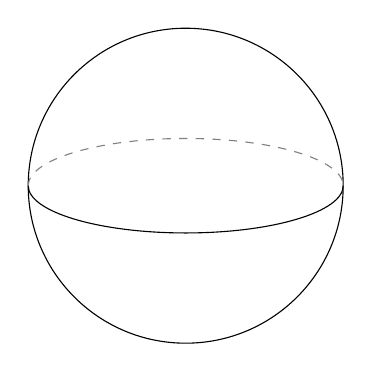
\begin{tikzpicture}
			% Draw a sphere
			\draw (0,0) circle (2cm);
			% Draw the equator
			\draw[thin] (-2,0) arc (180:360:2 and 0.6);
			% Draw the inside of the sphere
			\draw[dashed, gray] (-2,0) arc (180:0:2 and 0.6);
		\end{tikzpicture}
		\caption{A homeomorphic representation of the 2-sphere}
		\label{fig:2_sphere}
	\end{figure} \noindent
	The sphere has the property that all the loops at any point are homotopic, hence the
	fundamental group (at every point) of the sphere is the trivial group:
	\begin{equation}
		\forall p \in S^2: \pi_1(p) = \qty{[\gamma_{e, p}]}. \label{eq:fundamental_group_sphere}
	\end{equation}
\end{example}

\begin{example}[Cylinder \(S^1 \times \R\)]
	The cylinder \(C\) is defined as
	\begin{equation}
		C := \R \times S^1 \label{eq:cylinder}
	\end{equation}
	equipped with product topology.
	\begin{figure}[H]
		\centering
		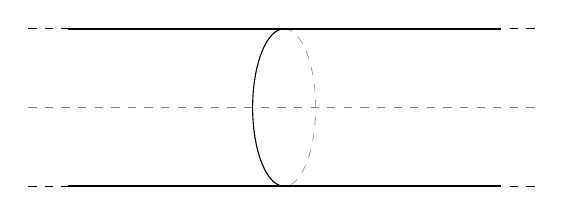
\begin{tikzpicture}
			\draw (0, 1) arc (90:270:0.4cm and 1cm);
			\draw[very thin, dashed, gray] (0, 1) arc (90:-90:0.4cm and 1cm);
			\draw[thick] (-2.75, 1) -- (2.75, 1);
			\draw[dashed] (-3.25, 1) -- (3.25, 1);
			\draw[dashed, gray] (-3.25, 0) -- (3.25, 0);
			\draw[dashed] (-3.25, -1) -- (3.25, -1);
			\draw[thick] (-2.75, -1) -- (2.75, -1);
		\end{tikzpicture}
		\caption{A homeomorphic representation of the cylinder}
		\label{fig:cylinder}
	\end{figure} \noindent
	A loop in $C$ can either go around the cylinder (\ie\ around its central axis) or not. If it does not, then it can be continuously deformed to a point (the identity loop). If it does, then it cannot be deformed to the identity loop (intuitively because the cylinder is infinitely long) and hence it is a homotopically different loop. The number of times a loop winds around the cylinder is called the \emph{winding number}. Loops with different winding numbers are not homotopic. Moreover, loops with different oreintations are also not homotopic. Hence, the fundamental group of the cylinder at any point is isomorphic to the additive group of integers:
	\begin{equation}
		\forall p \in C: \qty(\pi_1(p), \bullet_p) \grpIso (\Z, +). \label{eq:fundamental_group_cylinder}
	\end{equation}
\end{example}

\begin{example}[2-Torus \(S^1 \times S^1\)]
	The 2-torus \(T^2\) is defined as
	\begin{equation}
		T^2 := S^1 \times S^1 \label{eq:2_torus}
	\end{equation}
	equipped with product topology.
	\begin{figure}[H]
		\centering
		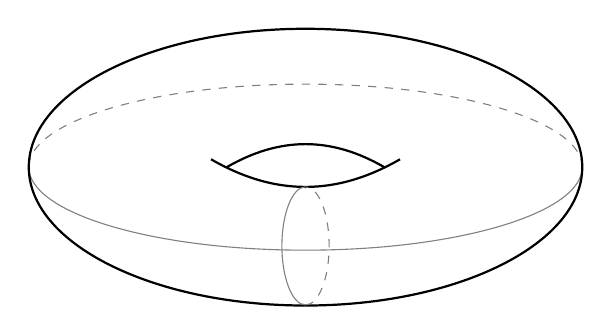
\begin{tikzpicture}
			\draw[thick] (-1,0) to[bend left] (1,0);
			\draw[thick] (-1.2,.1) to[bend right] (1.2,.1);
			\draw[gray] (100pt,0) arc (0:-180:100pt and 30pt);
			\draw[gray,dashed] (100pt,0) arc (0:180:100pt and 30pt);
			\draw[thick] (0,0) ellipse (100pt and 50pt);
			\draw[gray,dashed]  (0,-1.75) arc (-90:90:0.3 and 0.75);
			\draw[gray] (0,-1.75) arc (-90:-270:0.3 and 0.75);
		\end{tikzpicture}
		\caption{A homeomorphic representation of the 2-torus}
		\label{fig:2_torus}
	\end{figure} \noindent
	For the 2-torus, the fundamental group at any point is isomorphic to the additive group of integers squared:
	\begin{equation}
		\forall p \in T^2: \qty(\pi_1(p), \bullet_p) \grpIso (\Z \times \Z, +). \label{eq:fundamental_group_torus}
	\end{equation}
	Here the group operation is component-wise addition.
\end{example}

But still, the question remains: does a complete list of topological invariants exist \ie\ can we conclude that two spaces are homeomorphic if and only if they have the same topological invariants?

This problem is still open in topology and is known as the \emph{classification of topological spaces}.
